\documentclass[10pt]{article}
\usepackage[a4paper,margin=2cm]{geometry}
\usepackage{graphicx,booktabs,amsmath,amssymb,hyperref,xcolor,caption,subcaption}
\usepackage[numbers,sort&compress]{natbib}
\captionsetup{font=small}
\usepackage[skip=6pt]{parskip}

\title{Searching for online bin-packing heuristics\\ with LLM-guided evolution\\[4pt]
\large What the loop adds, what the model brings, and what the programs learn}
\author{Samuel Goh Jun Yang (A0259280Y), individual submission}
\date{Repository: \url{https://github.com/sayemuel/dsa4212_llm_binpacking_evolution}}

\begin{document}
\maketitle

\begin{abstract}
I built a small version of FunSearch, where a language model writes Python priority functions for
online bin packing, a simulator scores them, and good programs are shown back to the model in later
prompts. My simulator reproduces the published Best Fit and FunSearch numbers (3.98\% and 0.69\%
above the $L_1$ bound), so the rest of the results can be compared with the paper. With a budget of
300 to 800 proposals per run (about US\$0.0007 each), the evolutionary loop did not beat the simpler
approach of sampling proposals independently and keeping the best one. Sampling runs behave almost
exactly like independent draws from one fixed distribution, while every evolve run ended up outside
the range that model predicts, three better and three worse. Looking inside the programs, almost all
of the gain comes from one idea, avoiding leftovers of roughly 5 to 35\% of the bin. A three
parameter rule with that idea, tuned by plain grid search, does as well as the best LLM program on
validation and better on large test instances, but it breaks badly on other item distributions. Two
further findings surprised me. The stronger model at high effort mostly recalled FunSearch's
published heuristic from memory, and that heuristic loses to Best Fit on small instances because it
pays a fixed cost of about 10 to 17 bins whatever the instance size.
\end{abstract}

\section{Problem and motivation}
In online bin packing, items arrive one at a time and each must be placed immediately into a bin
with enough room, or into a new bin. The goal is to use as few bins as possible. Simple rules such as
First Fit and Best Fit \cite{johnson1973near,coffman2013binpacking} are fast and work reasonably well,
but no online rule is optimal on every input. FunSearch \cite{romera2024funsearch} showed that a
large language model (LLM) placed inside an evolutionary loop can write priority functions that beat
Best Fit on a given distribution, for example 0.68\% against 3.98\% excess bins on Weibull instances.
Later systems \cite{liu2024eoh,ye2024reevo,novikov2025alphaevolve,lange2025shinka} changed the
prompts, added reflection or improved the selection step, but most of them use thousands to millions
of LLM calls.

I picked this topic because it sits between two things I know from my degree, optimisation and
statistics, and one thing I had not done before, using an LLM as part of a search algorithm. In
class, a stochastic search method is usually compared against random search, and random search is
known to be a hard baseline to beat \cite{bergstra2012random}. I wanted to see whether the same is
true when the ``random'' proposals come from an LLM. With a total budget under US\$10, I asked three
questions. \textbf{Q1:} does the evolutionary loop add anything over independent sampling from the
same model with the same number of proposals? \textbf{Q2:} how do the choice of model and the
reasoning effort change the search? \textbf{Q3:} what do the programs that work actually do, and do
they still work on different sizes and distributions? I cared more about explaining the results than
about getting the single best number.

\section{Setup}
\subsection{Packing protocol, data and metric}
I follow FunSearch's protocol. A heuristic is a function \texttt{priority(item, bins)}. It receives
the item size and the remaining capacity of every bin the item fits in, and returns one score per
bin. The array has one slot per item, so an empty bin is always available. The simulator puts the
item in the highest scoring bin, with ties going to the oldest bin. The evolved code never decides
feasibility itself. The simulator removes bins that are too small, rejects outputs of the wrong
shape or with non-finite values, and checks that no bin is ever overfilled.

Item sizes for the main experiments come from a Weibull distribution (shape 3, scale 45), rounded
and clipped to $[1,100]$, with capacity $C=100$, as in FunSearch. The search only sees
\textbf{TRAIN}, five instances of 1\,000 items. \textbf{VALID} (five other instances of 1\,000 items)
is only used at the end of a run to choose its final program from its five best training programs.
Six \textbf{TEST} sets are never touched during the search: Weibull with 5\,000 items (FunSearch's
headline setting), 10\,000 items and 200 items, OR-Library style uniform sizes from 20 to 100 with
$C=150$ \cite{beasley1990orlib}, Weibull sizes with bigger bins ($C=150$), and Falkenauer style
``triplet'' instances with 501 items where every optimal bin holds exactly three items, so the
optimum is known \cite{falkenauer1996hybrid}. All instances come from fixed seeds that do not overlap
between splits.

The metric is the percentage of bins used above the lower bound $L_1=\lceil\sum_i s_i/C\rceil$, as in
FunSearch. I also implemented Martello and Toth's bound $L_2$ \cite{martello1990knapsack}, but it is
equal to $L_1$ on all my Weibull instances, so the excess is an upper bound on the true gap to the
optimum. Best Fit Decreasing, which sees all items in advance, is shown only as an offline reference.

\subsection{Two search modes}
\textbf{Evolve.} This follows FunSearch's design at a small scale. A program database has four
islands, each starting from Best Fit. For each proposal I pick an island at random and then two of its
programs, with softmax weights on their rank (temperature 2). The prompt shows the two programs
from worse to better with their training scores and asks for an improved version. The new program is
scored on TRAIN and added to the island it came from. Programs that make exactly the same decisions on
TRAIN are merged, keeping the shorter code, and the worse half of the islands is reset from the best
programs three times per run.

\textbf{Sample (the control).} Every prompt shows only the Best Fit seed and asks for something
better. No score is ever fed back, so the proposals are independent. Everything else is the same:
model, system prompt, evaluator, budget and final selection rule. Any difference between the two
modes is therefore the effect of the feedback loop.

\textbf{Models and budgets.} I used Claude Haiku 5.5 (US\$0.10 and \$0.50 per million input and
output tokens) and Claude Opus 5.5 (\$4 and \$20) through the Anthropic API, with reasoning effort
``low'' unless stated otherwise. The main comparison runs Haiku in both modes with three seeds of
300 proposals and three more seeds of 800 proposals. Opus gets 120 proposals per run (two evolve
seeds and one sample seed), and there is one high effort run for each model. Every proposal's code,
tokens, cost, latency and score is logged in \texttt{results/runs/*/proposals.jsonl}, which is what
made the later analyses in Section~\ref{sec:mech} possible without spending more money. Candidate
code runs in a separate Python process with a time limit, after a static check that it only imports
\texttt{numpy} and \texttt{math}.

\section{Results}
\subsection{Sanity check against FunSearch}
On the Weibull test instances with 5\,000 items, my Best Fit uses 3.98\% more bins than $L_1$ and
FunSearch's published heuristic (copied from the paper) uses 0.69\%. The paper reports 3.98\% and
0.68\% \cite{romera2024funsearch}. I take this as evidence that my protocol, instance generator and
metric are close enough to theirs for the numbers below to be comparable.

\subsection{Q1: does the evolutionary loop help?}
\begin{figure}[t]
\centering
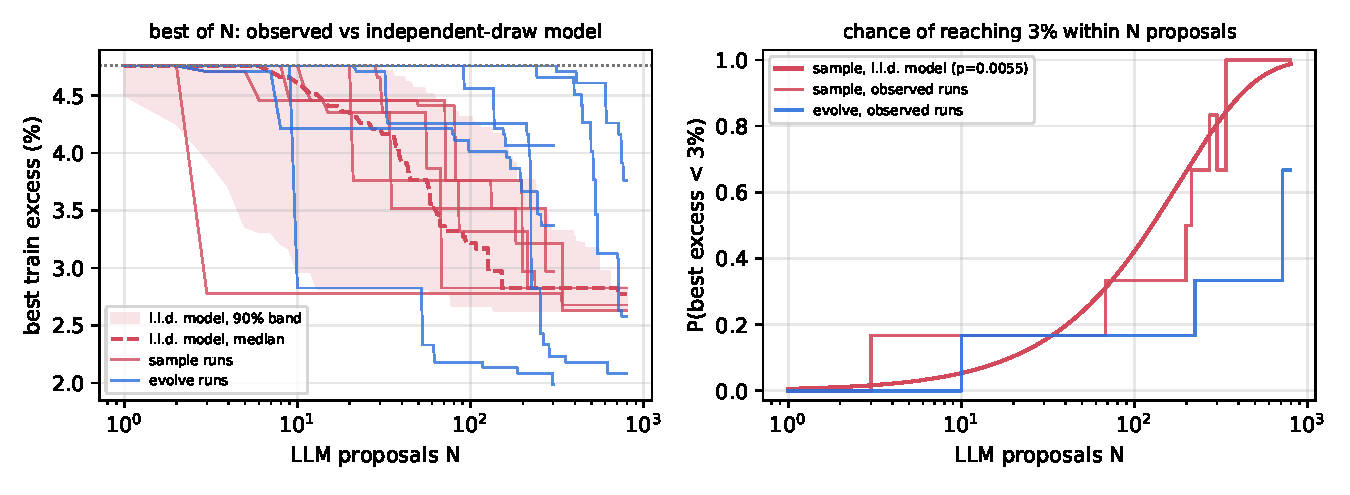
\includegraphics[width=\linewidth]{figures/bestofn.pdf}
\caption{Haiku at low effort. Left: best training excess so far for each run (thin lines), against
what I would expect if every proposal were an independent draw from the pooled distribution of all
3\,300 sample mode proposals (dashed median and shaded 90\% band, 2\,000 bootstrap replicates). The
dotted line is Best Fit. Right: chance that the best program so far is below 3\%, from the same model
and from the observed runs.}
\label{fig:bestofn}
\end{figure}

\textbf{Headline comparison.} Taking all six seeds per mode up to 300 proposals, the best training
excess under evolve was $\{4.06, 3.37, 1.98, 4.76, 4.66, 2.23\}$\% and under sampling
$\{2.82, 2.82, 2.97, 3.22, 2.78, 2.83\}$\%. A Mann-Whitney test finds no difference in location
($p=0.39$), but Levene's test finds a clear difference in spread ($p=0.004$). With only six runs per
arm, the smallest two-sided $p$ value a Mann-Whitney test can even produce is $2/\binom{12}{6}=0.002$,
so this test has little power and ``no significant difference'' should be read as ``no evidence
either way'', not as proof that the two are equal. After the final selection step on VALID, the
800 proposal runs give $2.82\pm0.77$\% for evolve and $2.79\pm0.15$\% for sampling, against 4.38\% for
Best Fit.

\textbf{A null model for sampling.} If sample mode proposals really are independent, the best score
after $N$ proposals is just the minimum of $N$ draws from one distribution. I estimated that
distribution from all 3\,300 Haiku sample proposals and bootstrapped the best of $N$ curve
(Figure~\ref{fig:bestofn}). The assumptions hold up well. The six sampling runs are consistent with
coming from the same distribution (Kruskal-Wallis $p=0.18$), the lag-one autocorrelation inside each
run is between $-0.04$ and $0.07$, and all six runs finish inside the model's 90\% band. The model's
median best at 300 proposals is 2.82\%, the same as the observed sampling runs. The distribution is
very skewed. 90\% of proposals are no better than Best Fit, only 0.55\% are below 3\%, and the best of
all 3\,300 is 2.63\%. This explains the right panel. Each proposal has roughly a 1 in 180 chance of
going below 3\%, so about 550 proposals are needed to be 95\% sure of getting there, and no amount of
sampling is likely to get much below 2.6\%.

\textbf{Evolve does not fit this model at all.} Every one of the six evolve runs finishes outside the
band. Three are worse than any sampling run would plausibly be (4.06, 3.37 and 3.76\%) and three are
better than the sampling floor (1.98, 2.08 and 2.58\%). So feedback changes the shape of the outcome
rather than its average. It lets a run build past the best single idea the model produces, but it can
also get stuck. Reading the logs, the stuck runs had islands full of small refinements of Best Fit
(around 4.6\%), and the prompts kept anchoring the model to tiny edits of those, so hundreds of
proposals went into improving the second decimal place. Under evolve, 49\% of proposals beat Best
Fit against 10\% under sampling, but that mostly reflects that evolve proposals are edits of parents
that are already better than Best Fit. My conclusion for Q1 is that at a few hundred proposals,
independent sampling is the more reliable choice, and evolution is a gamble with a higher ceiling.

\subsection{Q2: model and reasoning effort}
\begin{table}[t]
\centering\small
\begin{tabular}{lrrrrrr}
\toprule
Configuration & runs & proposals & beat BF & identical to BF & sel.\ valid (\%) & \$/proposal \\
\midrule
Haiku low, evolve   & 6 & 300/800 & 0.49 & 0.19 & $2.88\pm0.65$ & 0.0007 \\
Haiku low, sample   & 6 & 300/800 & 0.10 & 0.45 & $2.86\pm0.15$ & 0.0007 \\
Haiku high, evolve  & 1 & 150     & 0.03 & 0.59 & 4.23          & 0.0013 \\
Opus low, evolve    & 2 & 120     & 0.00 & 0.26 & 4.33          & 0.0102 \\
Opus low, sample    & 1 & 120     & 0.00 & 0.33 & 4.23          & 0.0093 \\
Opus high, evolve$^\dagger$ & 1 & 25 & 0.72 & 0.08 & 1.72       & 0.0423 \\
\midrule
Best Fit (seed) & & & & & 4.38 & \\
\bottomrule
\end{tabular}
\caption{Search statistics by configuration. ``Beat BF'' is the share of valid proposals with lower
training excess than Best Fit. ``Identical to BF'' is the share that pick the same bin as Best Fit in
all 1\,000 Best Fit states of the first training instance. ``Sel.\ valid'' is the validation excess
of each run's chosen program (mean $\pm$ s.d.\ over runs, pooling budgets 300 and 800).
$^\dagger$Stopped by the spending cap, and contaminated by recall (see text).}
\label{tab:search}
\end{table}

I expected the bigger model to do better, but it did not. Opus at low effort never beat Best Fit in 360
proposals, while Haiku, which is about 15 times cheaper per proposal, did so routinely
(Table~\ref{tab:search}). To understand why, I measured each proposal's \emph{disagreement rate}. I
replay the 1\,000 states that Best Fit visits on the first training instance and count how often the
proposal would choose a different bin (Figure~\ref{fig:dis}). A program that agrees with Best Fit
everywhere cannot possibly do better than it.

\begin{figure}[t]
\centering
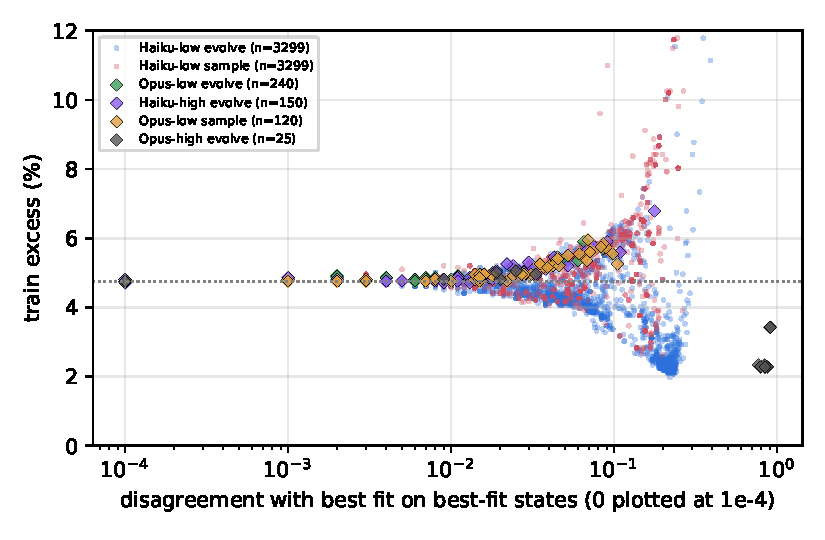
\includegraphics[width=0.6\linewidth]{figures/disagreement.pdf}
\caption{Each point is one valid proposal, showing its disagreement with Best Fit (log scale) against
its training excess. The dotted line is Best Fit. Points on the far left make the same choices as
Best Fit and so cannot improve on it.}
\label{fig:dis}
\end{figure}

The answer is that Opus at low effort was too cautious. Most of its proposals add small corrections,
such as a penalty of 0.01 to 0.03 on gaps below about 5\% of the bin, which almost never outweigh Best
Fit's own preference. Their median disagreement is 0.4\%, and about two thirds of them change fewer
than 1\% of decisions. Haiku at low effort proposes larger penalties over wider ranges (median
disagreement 3.4\% under evolve), and the improving programs sit at roughly 10 to 30\% disagreement.
Across all configurations, of the proposals that failed to beat Best Fit, 45\% changed no decision
at all and 55\% changed fewer than 1\%. Effort did not help in a simple way either. Haiku at high
effort became even more cautious (59\% identical to Best Fit, 3\% improving), while Opus at high
effort changed 79\% of decisions. Being bold is not enough by itself. About half of the Opus low
sample proposals changed more than 1\% of decisions and still never improved, because they mostly
changed how very small gaps are treated, and with integer item sizes those are close to exact fits
anyway. In Figure~\ref{fig:dis} these sit on an upper branch where more disagreement means a worse
score, separate from the lower branch of improving Haiku programs.

\textbf{Contamination.} The best single run (Opus at high effort, 1.72\% on validation) is not a
discovery. From its second proposal the model wrote that it was using ``the FunSearch-style
heuristic known to beat best fit on Weibull-like distributions'' and later that it was ``recalled from
memory''. Ten of its 25 programs contain the published formula, including its unusual step of
subtracting each bin's score from the next one. It then improved the recalled heuristic on 1\,000 item
instances by adding an override that always takes near-perfect fits (training excess 3.42\% to
2.28\%). Haiku never mentioned FunSearch in more than 5\,000 proposals, and none of its programs
uses that differencing step. Opus at low effort mentioned FunSearch 8 times without using the
formula. I report this run separately and do not count it as evidence that the search works. For
anyone using published benchmarks with LLM search, this is a real risk, because the model may have
seen the answer during training. The hybrid is still interesting on the test sets. It is slightly
worse than the original at large $n$ (0.83\% against 0.69\% at 5\,000 items) but roughly halves the
original's losses on small, uniform and triplet instances (7.8, 7.4 and 9.3\% against 13.9, 12.6 and
23.1\%, Table~\ref{tab:test}), which fits the fixed overhead story in Section~\ref{sec:overhead}.

\subsection{Q3: what the programs learn, and whether it transfers}\label{sec:mech}
\textbf{What ideas show up in the code.} To see which ideas the model tries, I tagged every valid
Haiku sample proposal by searching its code for a few patterns (Table~\ref{tab:ideas}). Sample mode is
the cleanest place to look because there is no feedback to bias which ideas appear. The tags are only
rough, since they match words in the code and docstrings, but one result is very clear. Programs that
mention a gap band or dead zone beat Best Fit 21.6\% of the time, against 0.9\% for programs that do
not. A bonus for exact or near-exact fits, the idea most people would try first, appears in two thirds
of proposals and is, if anything, slightly harmful. This is correlation within the model's own
output, not a controlled experiment, but it points straight at the mechanism.

\begin{table}[t]
\centering\small
\begin{tabular}{lrrrr}
\toprule
Idea found in the code & share & beat BF (with) & beat BF (without) & Fisher $p$ \\
\midrule
exact/near-fit bonus & 66\% & 8.8\% & 12.4\% & 0.001 \\
gap band / dead zone & 44\% & 21.6\% & 0.9\% & $<$0.001 \\
exponential or power & 21\% & 9.8\% & 10.1\% & 0.831 \\
special-cases the empty bin & 73\% & 12.0\% & 5.0\% & $<$0.001 \\
\bottomrule
\end{tabular}

\caption{Ideas found in the code of the 3\,299 valid Haiku low sample proposals (base rate of beating
Best Fit: 10.1\%). ``Share'' is the share of proposals with the tag. Tags are regular expressions on
the code, so they are approximate. Rarer tags (under 5\%) are left out.}
\label{tab:ideas}
\end{table}

\begin{figure}[t]
\centering
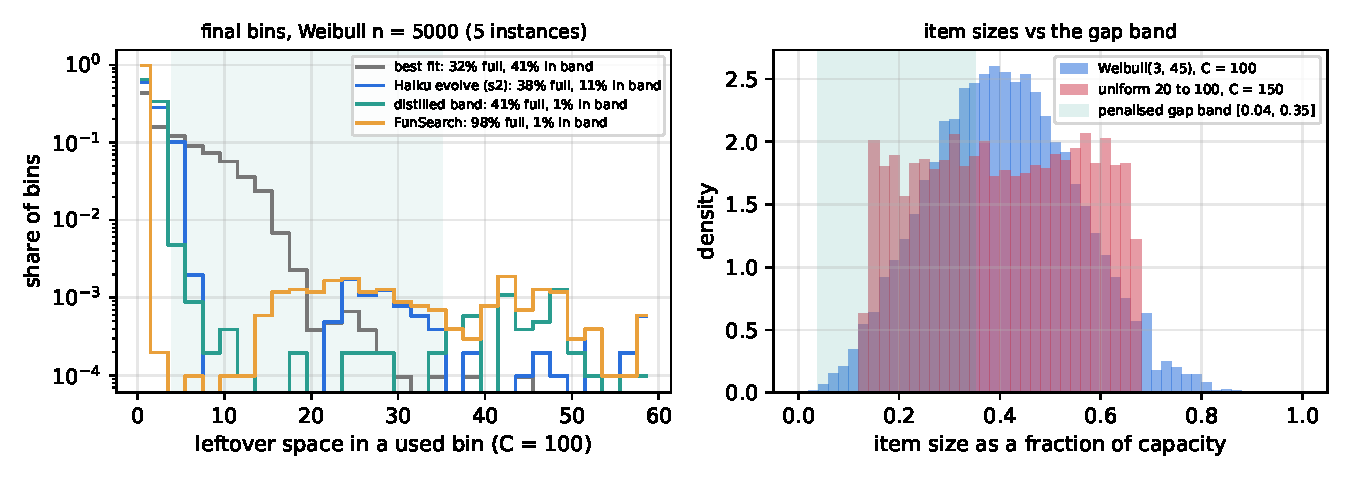
\includegraphics[width=\linewidth]{figures/leftovers.pdf}
\caption{Left: leftover space in every used bin at the end of packing five Weibull instances of
5\,000 items (log scale). The shaded area is the penalised band of the distilled rule. Right: item
size distributions of the Weibull training data and the uniform test data, as a fraction of capacity.}
\label{fig:leftovers}
\end{figure}

\textbf{What the bins look like.} Figure~\ref{fig:leftovers} shows the effect directly. Best Fit
ends with 41\% of its bins having a leftover between 4 and 35 units, and a mean leftover of 3.8
units. Under Weibull(3, 45) only 1.2\% of items are 10 or smaller and 9\% are 20 or smaller, so a
gap of that size is very unlikely to be filled later. The best Haiku program cuts the share of bins
in that band to 11\% and the distilled rule below 1\%, while the mean leftover drops to 1.6 and 1.4
units. They do not get rid of waste entirely. Instead they turn medium gaps into tiny ones of 1 to 3
units, which now make up over half of their bins. In effect the rule says: if putting this item here
would leave an awkward hole, open a new bin and keep this space for a bigger item that will fit more
tightly. FunSearch's heuristic goes much further and fills 98\% of its bins exactly.

\textbf{A three parameter version.} To test whether this one idea explains the gains, I wrote it as
a three parameter rule, Best Fit minus a penalty $c$ whenever the leftover lies in $[aC,bC]$. A 270
point grid search on TRAIN with no LLM picks $a=0.04$, $b=0.35$ and any $c\ge1$. A penalty of at
least 1 outweighs every Best Fit score difference, so the rule simply means ``avoid these gaps
whenever possible''. It ties the best Haiku program on VALID (2.21\%) and gets 1.41\% on 5\,000 item
Weibull instances and 1.27\% on 10\,000 item ones, better than every Haiku program
(Table~\ref{tab:test}). So the LLM found the right \emph{structure} but tuned its constants poorly,
and an ordinary parameter search did that part better and much more cheaply.

\begin{figure}[t]
\centering
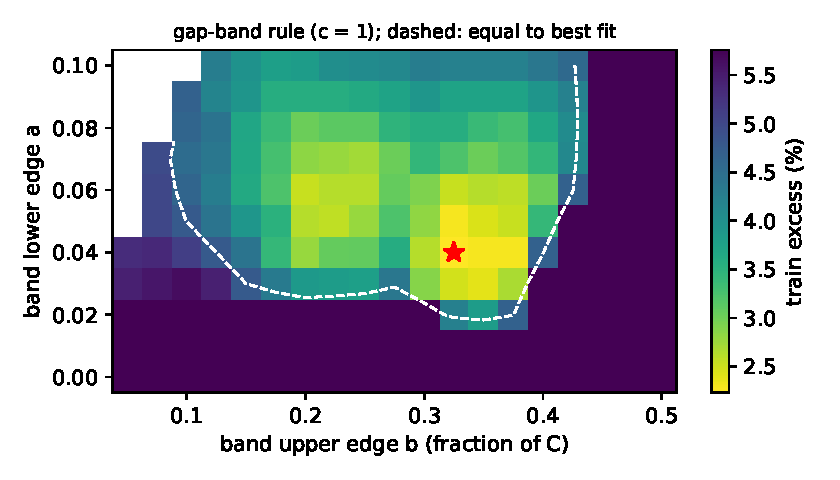
\includegraphics[width=0.6\linewidth]{figures/landscape.pdf}
\caption{Training excess of the gap band rule with $c=1$ on an $11\times19$ grid of $(a,b)$. Inside
the dashed line the rule beats Best Fit. The star marks the best cell.}
\label{fig:landscape}
\end{figure}

A finer grid (Figure~\ref{fig:landscape}) shows why the LLM had trouble getting there by small
edits. About half of the $(a,b)$ cells beat Best Fit, but the good region is split into two pockets,
one around $b=0.2$ and one around $b=0.33$, with a weaker strip in between. The finer grid's best
cell ($a=0.04$, $b=0.325$, 2.23\%) is almost the same as the coarse grid's, so I kept the original
parameters. The bottom rows are also informative. Once $a$ reaches 0.02 or less, the band starts to
penalise the tiny 1 to 2 unit leftovers that the good rules rely on, and the rule collapses.

\begin{table}[t]
\centering\scriptsize
\begin{tabular}{lrrrrrr}
\toprule
Method & weibull\_5k & weibull\_10k & weibull\_200 & uniform\_500 & weibull\_c150 & triplet\_501 \\
\midrule
first\_fit & 4.31 & 4.36 & 6.01 & 5.67 & 2.78 & 11.20 \\
best\_fit & 3.98 & 4.05 & 5.64 & 5.22 & 2.70 & 11.20 \\
funsearch\_or & 0.69 & 0.34 & 13.94 & 12.62 & 3.90 & 23.05 \\
best\_fit\_decreasing(offline) & 0.36 & 0.34 & 0.80 & 1.34 & 0.53 & 13.71 \\
gap\_band(distilled) & 1.41 & 1.27 & 6.20 & 10.39 & 4.06 & 10.30 \\
Haiku-high evolve b150 (n=1) & 3.76 & 3.77 & 5.64 & 4.87 & 2.70 & 11.26 \\
Haiku-low evolve b300 (n=3) & 2.44 \scriptsize[1.6,3.1] & 2.34 \scriptsize[1.4,3.2] & 5.04 \scriptsize[4.3,5.4] & 3.78 \scriptsize[3.3,4.2] & 2.30 \scriptsize[2.2,2.5] & 9.54 \scriptsize[6.8,11.0] \\
Haiku-low evolve b800 (n=3) & 1.91 \scriptsize[1.5,2.5] & 1.67 \scriptsize[1.4,2.2] & 5.90 \scriptsize[5.5,6.7] & 4.38 \scriptsize[3.5,5.7] & 2.20 \scriptsize[2.0,2.4] & 9.26 \scriptsize[7.8,10.8] \\
Haiku-low sample b300 (n=3) & 1.94 \scriptsize[1.6,2.2] & 1.81 \scriptsize[1.4,2.1] & 6.19 \scriptsize[5.2,6.9] & 4.61 \scriptsize[4.4,5.0] & 2.60 \scriptsize[2.4,2.7] & 8.00 \scriptsize[4.0,15.0] \\
Haiku-low sample b800 (n=3) & 2.27 \scriptsize[2.2,2.3] & 2.11 \scriptsize[2.0,2.2] & 4.89 \scriptsize[4.7,5.2] & 4.20 \scriptsize[4.0,4.5] & 2.53 \scriptsize[2.3,2.7] & 6.55 \scriptsize[4.0,11.1] \\
Opus-high evolve b60 (n=1) & 0.83 & 0.63 & 7.79 & 7.41 & 2.78 & 9.28 \\
Opus-low evolve b120 (n=2) & 4.06 \scriptsize[4.1,4.1] & 4.08 \scriptsize[4.1,4.1] & 5.67 \scriptsize[5.6,5.7] & 5.32 \scriptsize[5.3,5.4] & 2.70 \scriptsize[2.6,2.8] & 11.20 \\
Opus-low sample b120 (n=1) & 3.61 & 3.76 & 5.64 & 4.82 & 2.33 & 11.20 \\
\bottomrule
\end{tabular}
\caption{Held-out excess over $L_1$ (\%). Rows for evolved programs give the mean over seeds, with
[min, max] in brackets. Triplet instances have a known optimum of $n/3$ bins, so they measure the
true gap. ``b60'' is the Opus high run's planned budget; the spending cap stopped it after 25
proposals.}
\label{tab:test}
\end{table}

\textbf{Transfer.} Table~\ref{tab:test} shows that the specialised rules fail under distribution
shift. The distilled rule is \emph{worse} than Best Fit on uniform sizes (10.4\% against 5.2\%) and
with bigger bins (4.1\% against 2.7\%). The right panel of Figure~\ref{fig:leftovers} suggests why.
With uniform items on $C=150$, the smallest item is already 13\% of a bin and the sizes are spread
evenly, so a fixed band tuned to Weibull sizes no longer marks the gaps that are actually hard to
fill, and the rule keeps opening new bins it does not need. The Haiku programs have softer and smoother
penalties and transfer better. Every low effort Haiku configuration beats Best Fit on average on
uniform sizes (3.8 to 4.6\% against 5.2\%), with bigger bins (2.2 to 2.6\% against 2.7\%) and on
triplets, though the spread on triplets is huge (4.0 to 15.0\%). On small Weibull instances they are
mixed (4.3 to 6.9\% against 5.6\%). The pattern I find most interesting is that the three best rules
on large Weibull instances (FunSearch's heuristic, the Opus hybrid built from it, and the distilled
rule) are also the three worst on uniform sizes. Being very good on one distribution seems to cost
robustness. A smaller surprise is that triplets are hard even for offline sorting. Best Fit Decreasing
(13.7\%) is worse than online Best Fit (11.2\%), because putting all the large items first breaks up
the exact triples.

\begin{figure}[t]
\centering
\begin{subfigure}{0.49\linewidth}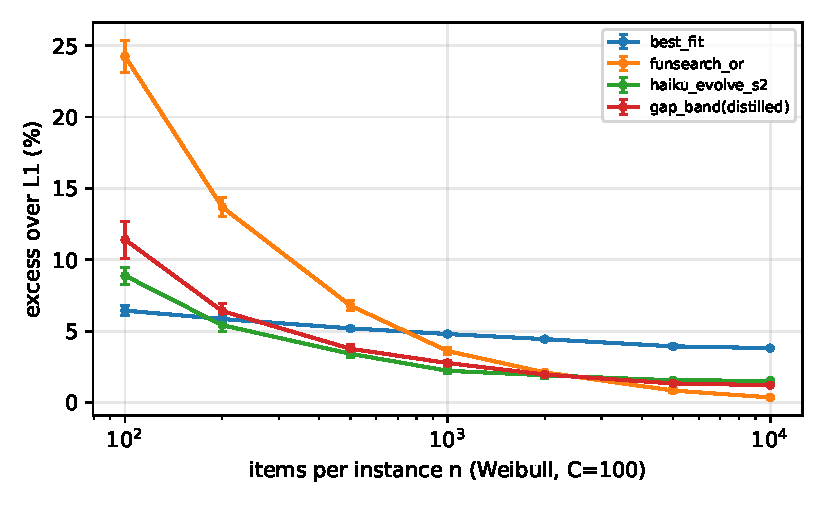
\includegraphics[width=\linewidth]{figures/scale.pdf}\end{subfigure}
\begin{subfigure}{0.49\linewidth}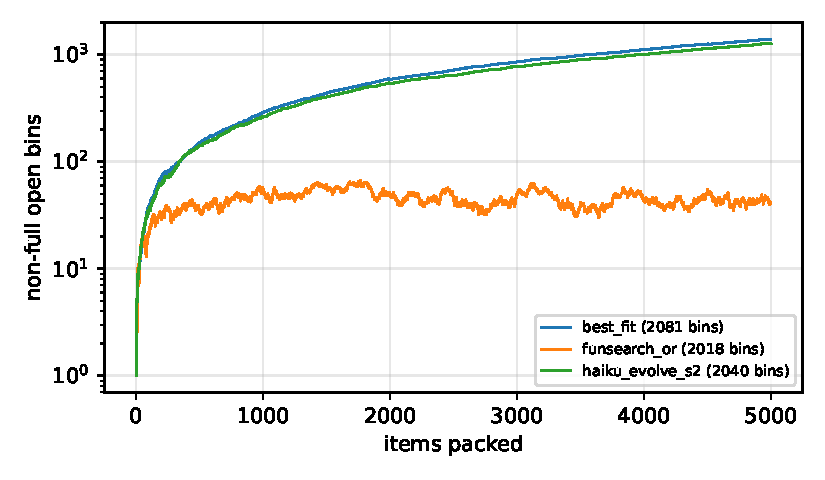
\includegraphics[width=\linewidth]{figures/openbins.pdf}\end{subfigure}
\caption{Left: excess against the number of items (Weibull, $C=100$; error bars are standard errors over
instances). Right: number of opened but not yet full bins while packing one Weibull instance of 5\,000
items.}
\label{fig:scale}
\end{figure}

\textbf{Why FunSearch's heuristic needs long instances.}\label{sec:overhead} Percentages hide what
is going on, but counting extra bins makes it clear (Figure~\ref{fig:scale}). Best Fit's extra bins
grow in proportion to $n$ (2.6, 19.4 and 153.5 extra bins at 100, 1\,000 and 10\,000 items), a steady
loss of about 1.5\% of capacity. FunSearch's heuristic pays a nearly constant 10 to 17 extra bins at
every size from 100 to 10\,000. The open bin trace shows how. Best Fit leaves hundreds of bins with
small unusable gaps (about 700 not yet full bins on average), while FunSearch's rule keeps a pool of
only about 44 partly filled bins and fills almost every other bin exactly. In a long stream that pool
eventually gets filled and costs almost nothing, but in a short instance it is mostly still open at
the end. The two rules cross between 500 and 1\,000 items. A metric averaged over long instances
rewards strategies with a large fixed cost, and this is easy to miss if only percentages are
reported.

\subsection{Cost of discovery and cost of use}
The whole study made 7\,135 proposals using 6.5M input and 7.9M output tokens, for US\$9.10 in
total (not counting five smoke test calls). A 300 proposal Haiku run costs about \$0.19 and takes 13
to 19 minutes with two requests in parallel, while 120 Opus proposals at low effort cost about \$1.2.
Opus at high effort costs \$0.042 per proposal, four times as much as at low effort, mostly because
it writes about five times more output. All the analyses in Section~\ref{sec:mech} ran on my laptop
with no API calls. Using the heuristics is cheap. The evolved programs pack 5\,000 items in under a
second, against about 0.1\,s for Best Fit. Only 2 of the 7\,135 proposals were invalid (one type error
and one with non-finite scores, both caught by the evaluator). So the hard part was never writing
valid code, it was coming up with a change that actually helped.

\section{Discussion and limitations}
\textbf{What I think the experiments show.} First, at a few hundred proposals, independent sampling
is a strong baseline. It matched evolution on average with far less variance, much like random search
in hyper-parameter tuning \cite{bergstra2012random}. Second, a proposal's value depends a lot on how
much it actually changes. Most failed proposals change almost nothing, and model size and effort
affect this in ways I did not expect. Third, the successful programs share one mechanism, and once
that mechanism is written down, a classical parameter search tunes it better than the LLM did.
Fourth, rules that are very good on one distribution, including FunSearch's, give up robustness, and
in FunSearch's case the size dependence is explained by a fixed overhead.

\textbf{What I am less sure about.} The high effort runs are single seeds, and the Opus high run is
short (25 proposals) and contaminated, so I do not try to rank the models. My budgets are four to
five orders of magnitude smaller than FunSearch's, and the evolve versus sample comparison could
change with more proposals or larger populations. The prompt design (two parents with scores) is
only one option, and a reflection step \cite{ye2024reevo} or an explicit instruction to make bigger
changes might reduce the caution problem. VALID has only five instances, so choosing among close
finalists is noisy, and there is some selection bias. For example, the best evolve program scored
1.98\% on TRAIN but 2.26\% on VALID. Finally, the excess is measured against $L_1$, which is only a
lower bound except on the triplet instances.

\textbf{A cheap improvement.} Two things follow directly from the findings. Before spending time
evaluating a proposal, the loop could check its disagreement with its parent and reject proposals
that change almost nothing. And instead of asking the LLM for finished programs, it could ask for a
\emph{structure} with free constants, which a numerical optimiser then tunes, as in my distillation
experiment.

\section{Reflection}
Coming into this project I mostly thought of LLMs as tools for writing text or code, not as parts of
an optimisation algorithm, and I treated FunSearch's result as something that would carry over if I
copied the method. Doing it at a small scale changed how I see it. The part that mattered most was
not the LLM but the experimental design around it. Without the sample mode control, I would have
reported the best evolve run (1.98\%) and concluded that evolution works. Without the null model I
would not have noticed that the two modes differ in shape and not in average. This is basically the
lesson from statistics classes about needing a baseline and a model of chance, but I had not seen it
matter this much in a real experiment before.

Some results went against my expectations, and they were the most interesting part of the work.
I expected Opus to beat Haiku and higher effort to help, and neither happened in a simple way. I
expected the evolved programs to be hard to interpret, but almost all of them came down to one idea
that fits in one line. I did not expect to find contamination at all, and it only showed up because
every proposal's explanation was logged and checked, not just its score. That changed how I would read
papers that use well known benchmarks with LLMs.

The budget was a deliberate choice. Running the search through the Anthropic API meant I had to
decide how much to spend, and I weighed three options: a few dollars, under US\$10, or around US\$50 to 60, which would have allowed
many more Opus runs. None of these amounts is life changing, and for what is probably my last NUS
assignment it was tempting to just spend more. I decided against it because I did not want the
project to become pay to win, where the result mostly reflects how much compute I bought. I wanted it
to be about learning and making the most of limited resources. At the same time I could see what a
few dollars on Opus would add, so I spent them where they answered a specific question, the model
comparison and the high effort runs, and used the cheap model everywhere else. Every run had a
spending cap and every proposal was logged, so all the later analysis could be done offline for
free. This turned out to be one of the more useful lessons of the project. The most expensive option
is not automatically the best one, and in my internships I saw full timers on long term projects
treat cost control and planning as part of the engineering work, not something added at the end.
With how much AI compute costs today, I think that matters even more.

If I did this again, I would spend the budget on more seeds of shorter runs instead of a
few long ones, since the main uncertainty in Q1 comes from having only six runs per arm, and I would
compute disagreement during the search instead of afterwards.

\section{Conclusion}
A small FunSearch-style loop can find online packing rules that beat Best Fit for about US\$0.20 per
run with Haiku. In my controlled comparisons, independent sampling was as good as evolution on
average and much more predictable, and almost all of the gain came from one simple idea that the LLM
proposed and a grid search then tuned better. The strongest model's best result came from memory
rather than search. Looking at decisions (disagreement) and absolute extra bins, not only percentage
scores, is what explained most of these behaviours.

\bibliographystyle{plainnat}
\bibliography{references}

\appendix
\section{Prompts and settings}\label{app:prompts}
All prompts are verbatim in \texttt{code/evolve.py} and saved with every run in
\texttt{results/runs/*/config.json}. \textbf{System prompt} (both modes): the model is told it is an
expert in combinatorial optimisation and given the online problem, the signature
\texttt{priority(item, bins)}, the facts that \texttt{bins} contains only feasible bins in creation
order and always includes an empty bin, that the highest score wins with ties going to the earliest
bin, and that only \texttt{numpy} and \texttt{math} may be used, with no I/O, randomness or state. It
is asked for at most three sentences of explanation and exactly one Python code block.
\textbf{Evolve user prompt:} ``Below are previous versions of the priority function, ordered from
worse to better. Score = average percentage of bins used above the lower bound
ceil(sum(items)/capacity) on the evaluation instances (lower is better).'' This is followed by
\emph{Version 0 (excess = \ldots\%)} and \emph{Version 1}, each with its code, and then ``Write
version 2: an improved priority function with a lower excess. You may combine ideas from the
versions above or try something new.'' \textbf{Sample user prompt:} ``Here is a baseline
heuristic:'' followed by the Best Fit code and ``Write a new priority function that packs items into
fewer bins than this baseline.'' \textbf{Settings:} \texttt{max\_tokens} 16\,000, adaptive thinking
(the API default), effort \texttt{low} or \texttt{high}, no sampling parameters, 2 concurrent
requests per run, 4 islands of at most 20 programs, 2 programs per prompt, rank softmax temperature
2, 3 island resets, and the top 5 training programs re-scored on VALID. Spending caps per run: Haiku
\$0.60, Opus \$1.70, Opus high \$1.00, Haiku high \$0.40 (phase 1 ran without a cap).
\textbf{Exploratory analyses:} \texttt{code/explore.py} produces Figures~\ref{fig:bestofn},
\ref{fig:leftovers} and \ref{fig:landscape} and Table~\ref{tab:ideas} from the saved runs.
\end{document}
